\documentclass{beamer}
%
% Choose how your presentation looks.
%
% For more themes, color themes and font themes, see:
% http://deic.uab.es/~iblanes/beamer_gallery/index_by_theme.html
%
\mode<presentation>
{
  \usetheme{Madrid}      % or try Darmstadt, Madrid, Warsaw, ...
  \usecolortheme{default} % or try albatross, beaver, crane, ...
  \usefonttheme{default}  % or try serif, structurebold, ...
  \setbeamertemplate{navigation symbols}{}
  \setbeamertemplate{caption}[numbered]
} 

\usepackage{polski}
\usepackage[utf8]{inputenc}

\title[Analiza online strumieni danych]{Analiza online strumieni danych}														\subtitle{Praca Magisterska napisana pod kierunkiem dra Jakuba Lemiesza}
\author[A. Wilczak]{Adam Wilczak}
\institute[]{Politechnika Wrocławska, Wydział Podstawowych Problemów Techniki
}
\date{Wrocław, 2017}

\begin{document}

\begin{frame}
  \titlepage
\end{frame}

% Uncomment these lines for an automatically generated outline.
%\begin{frame}{Outline}
%  \tableofcontents
%\end{frame}

\section{Wprowadzenie}

\begin{frame}{Przedstawienie problemu}

\begin{block}{Problem zliczania unikalnych elementów w strumieniach danych}
\begin{itemize}
\item Rozpatrujemy strumień danych w którym elementy mogą się powtarzać z nieznaną częstotliwością
\item Chcemy wiedzieć ile unikalnych elementów znajduje się w strumieniu w danym momencie
\item Możemy szacować wynik z kontrolowanym błędem
\end{itemize}
\end{block}
\begin{block}{Możliwe rozwiązania}
	\begin{itemize}
		\item Przetrzymujemy każdy napotkany w strumieniu nowy element - potrzeba $O(n)$ pamięci
		\item Szacujemy $n$ z pewnym kontrolowanym błędem, ale korzystamy ze struktur potrzebujących znacznie mniej pamięci
		\item Algorytmy operujące na szkicach danych - MinCount, HyperLogLog
	\end{itemize}
\end{block}
\end{frame}

\begin{frame}{Szkice danych}
\begin{block}{Czym są szkice danych?}
	\begin{itemize}
		\item Struktura reprezentująca dane ze strumienia wejściowego
		\item Zazwyczaj elementy wejściowe są haszowane i w szkicu przetrzymujemy hasze
		\item Szkice różnią się w zależności od algorytmu
	\end{itemize}
\end{block}
\end{frame}

\begin{frame}{Probability}
\begin{block}{Generation of plane trees}
\centering
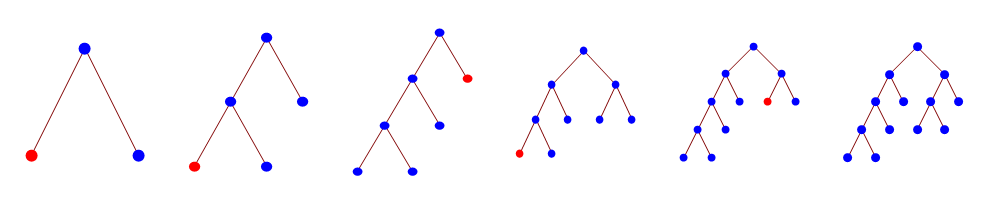
\includegraphics[width=0.95\textwidth]{Trees02}
\end{block}

\section{Basic properties}

\begin{block}{Basic formula}
For $t \in T_n$ we have
$$
\Pr[T_n = t] = \prod_{v\in t^o} \frac{1}{\Delta(v)-1}
$$
where $t^o$ is the set of interval nodes of $t$, $\Delta(v)$ is the number of leaves of a tree rooted at $v$.
\end{block}

\end{frame}

\begin{frame}{Probability - II}
\textbf{Remark}: generate randomly binary search tree from random permutation, make "de-labelization"; we get the same probability model.

\begin{block}{Recurrence}
If $t = t_1 \star t_2 \in T_n$, then
$$\Pr[T_n=t] = \frac{1}{n-1} \Pr[T_{\Delta(t_1)}=t_1] \Pr[T_{\Delta(t_2)}=t_2]$$
where $\Delta(s)$ is the number of leaves in $s$
\end{block}

\begin{block}{Connection between $S$ and $T$}
$$\Pr[S_n = s] = card([s]_\sim) \cdot \Pr[T_n = t], \quad t\in [s]_\sim$$
\end{block}

\end{frame}

\begin{frame}{Symmetries}

\begin{definition}
  $sym(t)$ = the number of non-leaf (internal)
nodes $v$ of tree $t$ such that the two subtrees stemming from $v$ are isomorphic.
\end{definition}

\begin{block}{Basic property}
$$
  card([s]_\sim) = 2^{n - 1 - sym(s)}
$$
\end{block}
\begin{block}{Basic recurrence}
$$
  sym(s_1\star s_2) = 
	\begin{cases}
	sym(t_1) + sym(t_2) + 1 &: t_1   =  t_2\\
	sym(t_1) + sym(t_2)     &: t_1 \neq t_2
	\end{cases}
$$
\end{block}

\end{frame}

\section{Gererating Functions}


\begin{frame}{Generating functions}

\begin{block}{Two basic generating functions}
\begin{itemize}
\item $F(u,z) = \sum_{t\in T} \Pr[T=t] u^{sym(t)} z^{|t|}$
\item $B(u,z) = \sum_{t\in T} \Pr[T=t]^2 u^{sym(u)} z^{|t|-1}$ 
\end{itemize}
\end{block}

% Commands to include a figure:
%\begin{figure}
%\includegraphics[width=\textwidth]{your-figure's-file-name}
%\caption{\label{fig:your-figure}Caption goes here.}
%\end{figure}

\begin{theorem}Let $f(u,z) = \frac{F(u,z)}{z}$. Then
$$
\frac{\partial  f(u,z)}{\partial z} = f(u,z)^2 + (u-1)B(u^2,z^2)
$$ 
\end{theorem}
(Riccati differential equation)
\end{frame}

\begin{frame}{Number of symmetries}
\begin{definition}
$$\mathcal{E}(z) = \sum_{n\geq 1} \mathbb{E}[sym(S_n)]z^n$$
\end{definition}

\begin{theorem}
Let $B(z) = \sum_{t\in T} \Pr[T=t]^2 z^{|t|-1}  \quad (= \sum_n b_n z^n)$. Then
$$
  \mathcal{E}'(z) = \frac{2\mathcal{E}(z)}{z(1-z)} + B(z^2)
$$
\end{theorem}

We should know the behavior of $B(z)=\sum_{n}b_nz^n$. We can calculate $b_1,b_2,b_3,\ldots$:
$$
1,1,\frac{1}{2},\frac{2}{9},\frac{13}{144},\frac{7}{200},\frac{851}{64800},\frac{13}{2700},\frac{1199}{691200},\frac{2071}{3359232}
$$
\end{frame}

\begin{frame}{Extraction of coefficients of function $B(z)$}
We put
$$
  C(z) = z B(z)
$$
\begin{block}{Differential equation}
$$
  C(z) - zC'(z) + z^2 C''(z) = C^2(z)
$$
\end{block}
\begin{block}{Recurrence}
$$
  c_n = \frac{1}{(n-1)^2} \sum_{k=1}^{n-1} c_k c_{n-k}
$$
\end{block}
\end{frame}

%%%%%%%%%%%%%%%%%%%%%%%%%%%%%%%%%%%%%%%%%%%%%%%%%%%%%%%%%%%%%%%%%%%%%%%%%%%%%%
\section{Extraction}

\begin{frame}{Solution of recurrence}
\begin{block}{Recurrence}
$$
  c_n = \frac{1}{(n-1)^2} \sum_{k=1}^{n-1} c_k c_{n-k}
$$
\end{block}

Numerical computations: $b_n = c_{n+1} \approx (\frac{1}{3.14})^n \cdot 6 n$
\pause
\begin{alertblock}{SOLUTION !!!}
H-H Chern, M. Fernández-Camacho, H-K. Hwang, and
C. Martinez, \textit{Psi-series method for equality of random
trees and quadratic convolution recurrences}, 2012: 
$$
  b_n = \rho^n\left(6 n - \frac{22}{5} + O(n^{-5})\right)
$$
where $\rho = 0.3183843834378459\ldots$.
\end{alertblock}
\end{frame}

\begin{frame}{Solution of differential equation}
\begin{itemize}
\item we defined: $\mathcal{E}(z) = \sum_{n\geq 1} \mathbb{E}[sym(S_n)]z^n$
\item we know that: $\mathcal{E}'(z) = \frac{2\mathcal{E}(z)}{z(1-z)} + B(z^2)$
\item we know a lot about $B(z) = \sum_n b_n z^n$
\end{itemize}

\begin{theorem}
$$
\mathrm{E}[sym(S_n)] = n \sum_{k=1}^{\left\lfloor \frac{n+1}{2}\right\rfloor}
\frac{b_k}{(2k-1)k(2k+1)} + (-1)^{n+1} b_{\left\lfloor \frac{n+1}{2}\right\rfloor}
$$
hence
$$
\mathrm{E}[sym(S_n)] = n\cdot (0.3725463659 \pm 10^{-10})
$$ 
\end{theorem}

\end{frame}

\section{Applications}

\begin{frame}{Application - compression}
\begin{columns}
\begin{column}{0.6\textwidth}
We know that $\mathrm{E}[sym(S_n)] \approx 0.3725 \cdot n$ 

\begin{block}{Simple compression algorithm}
If you find a symmetric inner node, replace one of its sub-trees by a pointer.
Let $size(S_n)$ denote the size of generated structure.
\end{block}
$$
  \mathbb{E}[size(S_n)] = n \sum_{k=1}^{\left\lfloor \frac{n+1}{2}\right\rfloor}
\frac{b_k}{(2k-1)(2k+1)}
$$
$$ 
\approx  0.4190 \cdot n
$$
\end{column}
\begin{column}{0.4\textwidth}
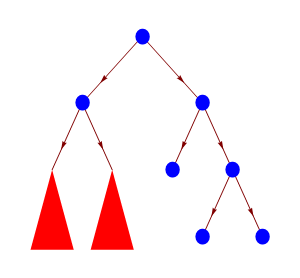
\includegraphics[width=0.8\textwidth]{Trees03} \\
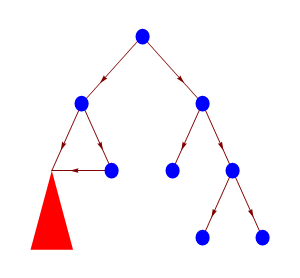
\includegraphics[width=0.8\textwidth]{Trees04}
\end{column}
\end{columns}
\end{frame}


\begin{frame}{Application - entropy}
We know that
\begin{itemize}
\item $H[S_n] = H[T_n] - H[T_n|S_n]$
\item $H[T_n] = \log_2(n-1) + 2 n \sum_{k=2}^{n-1} \frac{\log_2(k-1)}{k(k+1)}$
\item $2 \sum_{k=2}^{n-1} \frac{\log_2(k-1)}{k(k+1)} \approx 1.736$ (for $n\geq 10^5$)
\item $H[T_n|S_n] = \ldots = \sum_{s\in S_n} \Pr[S_n=s]\log_2(card([s]_\sim)) = \ldots
n-1-E[sym(T_n)]$
\end{itemize}

\begin{theorem}
$$
  \lim_{n\to\infty} \frac{H[S_n]}{n} = 1.109...
$$
\end{theorem}
\end{frame}

%%%%%%%%%%%%%%%%%%%%%%%%%%%%%%%%%%%%%%%%%%%%%%%%%%%%%%

\begin{frame}{This is the end}

\begin{figure}
\centering
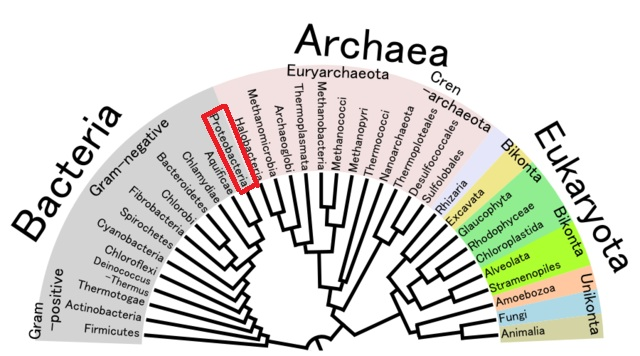
\includegraphics[width=0.5\textwidth]{PhylogeneticTree}
\caption{Phylogenetic (evolutionary) Tree}
\end{figure}

\begin{block}{}
\begin{center}
{\Huge Thank You}
\end{center}
\end{block}

\end{frame}

\end{document}